\documentclass[10pt]{article}

\usepackage[mode=buildnew,subpreambles=true]{standalone}
\input{preamble}

\title{\bf Short summary}
\author{Yann-Edwin Keta}
\date{November 12th, 2019}

\begin{document}

\maketitle

\section{Model}

We consider an ensemble of $N$ spherical ABPs $i$, with positions $\underline{r}_i$ and orientations $\theta_i$, which are self-propelled along the direction $\underline{u}_i \equiv (\cos(\theta_i), \sin(\theta_i))$. We have the following dimensionless equations of motion \cite{nemoto_optimizing_2019},
\begin{equation}
\begin{aligned}
\dot{\underline{r}}_i(t) &= \frac{1}{3} \frac{\sigma}{l_p} \tilde{\underline{F}}_{i, ex}(t) + \underline{u}_i(t) + \sqrt{\frac{2}{3}\frac{\sigma}{l_p}} \underline{\eta}_i(t),\\
\dot{\theta_i}(t) &= \sqrt{2\frac{\sigma}{l_p}} \xi_i(t),
\end{aligned}
\label{EOM}
\end{equation}
where $\tilde{\underline{F}}_{i, ex}$ is the total force applied on particle $i$ deriving from a WCA potential, $l_p$ is the persistence length, $\sigma$ is the particle diameter, and $\underline{\eta}_i \equiv (\eta_{x, i}, \eta_{y, i})$ and $\xi_i$ are independent Gaussian white noises of unit variance and zero mean.\\

We define the normalised rate of active work,
\begin{equation}
w(t_0; \tau) = \frac{1}{N \tau} \, (S)\int_{t_0}^{t_0 + \tau} \sum_{i=1}^{N} \underline{u}_i(t) \cdot \text{d}\underline{r}_i(t) = \frac{1}{2 N \tau \, \Delta t} \sum_{t=0}^{\tau - 1} \sum_{i=1}^n \left(\underline{u}(\theta_{i, t_0 + t + 1}) + \underline{u}(\theta_{i, t_0 + t})\right) \cdot \left(\underline{r}_{i, t_0 + t + 1} - \underline{r}_{i, t_0 + t}\right),
\end{equation}
which we can write as a sum of three terms,
\begin{equation}
\begin{aligned}
w_f(t_0; \tau) &= \frac{1}{2 N \tau} \sum_{t=0}^{\tau - 1} \sum_{i=1}^n \left(\underline{u}(\theta_{i, t_0 + t + 1}) + \underline{u}(\theta_{i, t_0 + t})\right) \cdot \frac{1}{3} \frac{\sigma}{l_p} \tilde{\underline{F}}_{i, ex, t_0 + t},\\
w_{\theta}(t_0; \tau) &= \frac{1}{2}\left(1 + \frac{1}{N\tau} \sum_{t=0}^{\tau - 1} \sum_{i=1}^N \cos(\theta_{i,t_0 + t  + 1} - \theta_{i,t_0 + t})\right),\\
w_{\eta}(t_0; \tau) &= \frac{1}{2N \tau} \sum_{t=0}^{\tau - 1} \sum_{i=1}^N \left(\underline{u}(\theta_{i,t_0 + t  + 1}) + \underline{u}(\theta_{i, t_0 + t})\right) \cdot \sqrt{\frac{2}{3} \frac{\sigma}{l_p} \frac{1}{\Delta t}} \, \underline{\eta}_{i, t_0 + t + 1},
\end{aligned}
\end{equation}
respectively the \textit{force}, \textit{orientation}, and \textit{noise} part of the active work.\\

We also define an order parameter,
\begin{equation}
\underline{\nu}(t) = \frac{1}{N} \sum_{i=1}^N \underline{u}(\theta_i(t)),
\end{equation}
with mean and correlations \footnote{Refer to appendix E of \cite{nemoto_optimizing_2019} for the derivation of the order parameter norm dynamics which we use to infer the corresponding results of equation \ref{meanVarOrder}.}
\begin{equation}
\begin{aligned}
\left<\underline{\nu}(t_0)\right> &= 0,\\
\left<|\underline{\nu}(t_0)|\right> &= \frac{1}{\sqrt{2N}},\\
\left<\delta \underline{\nu}(t_0 + \tau) \cdot \delta\underline{\nu}(t_0)\right> &= \frac{1}{N} \exp\left(-\frac{\sigma}{l_p}\tau\right),\\
\left<\delta |\underline{\nu}|(t_0 + \tau) \, \delta |\underline{\nu}|(t_0)\right> &= \frac{1}{4N} \exp\left(- 2\frac{\sigma}{l_p} \tau\right),
\end{aligned}
\label{meanVarOrder}
\end{equation}
in the absence of symmetry breaking.

\section{One-particle quantities}

We check our algorithm and set benchmarks by considering the \textit{free} or \textit{single particle} case, $\tilde{\underline{F}}_{i, ex} = 0$.\\

We can analytically derive the mean squared displacement,
\begin{equation}
\left<(\underline{r}(t_0 + \Delta t) - \underline{r}(t_0))^2\right> = \frac{l_p}{\sigma}\left(\Delta t + \frac{l_p}{\sigma}\left(\exp\left(-\frac{\sigma}{l_p} \Delta t\right) - 1\right)\right) + \frac{4}{3} \frac{\sigma}{l_p} \Delta t.
\end{equation}
and the active work mean and correlations
\begin{equation}
\begin{aligned}
\left<w(t_0; \tau)\right> &= 1,\\
\forall \tau \geq \tau_0,~ \left<\delta w(t_0; \tau_0) \delta w(t_0; \tau)\right> &= \frac{2}{3} \frac{\sigma}{l_p} \frac{1}{\tau},\\
\forall \tau \geq \tau_0,~ \left<\delta w(t_0; \tau_0) \delta w(t_0 + \tau; \tau_0)\right> &= 0.
\end{aligned}
\end{equation}
These theoretical predictions match the numerical results.

\section{Active work covariances}

We argue that
\begin{equation}
\left<\delta w(t_0; \tau_0) \delta w(t_0 + \tau; \tau_0)\right> \approx \left<\delta w_f(t_0; \tau_0) \delta w_f(t_0 + \tau; \tau_0)\right> + \left<\delta w_{\eta}(t_0; \tau_0) \delta w_f(t_0 + \tau; \tau_0)\right>,
\end{equation}
since that the fluctuations of the orientation part of the active work are negligible for low integration time steps, and that the orientational and translational noises are independent.\\

We plot the covariances between the different part of the active work with a delay $\tau$ in figure \ref{crossCor}.

\begin{figure}[H]
\centering
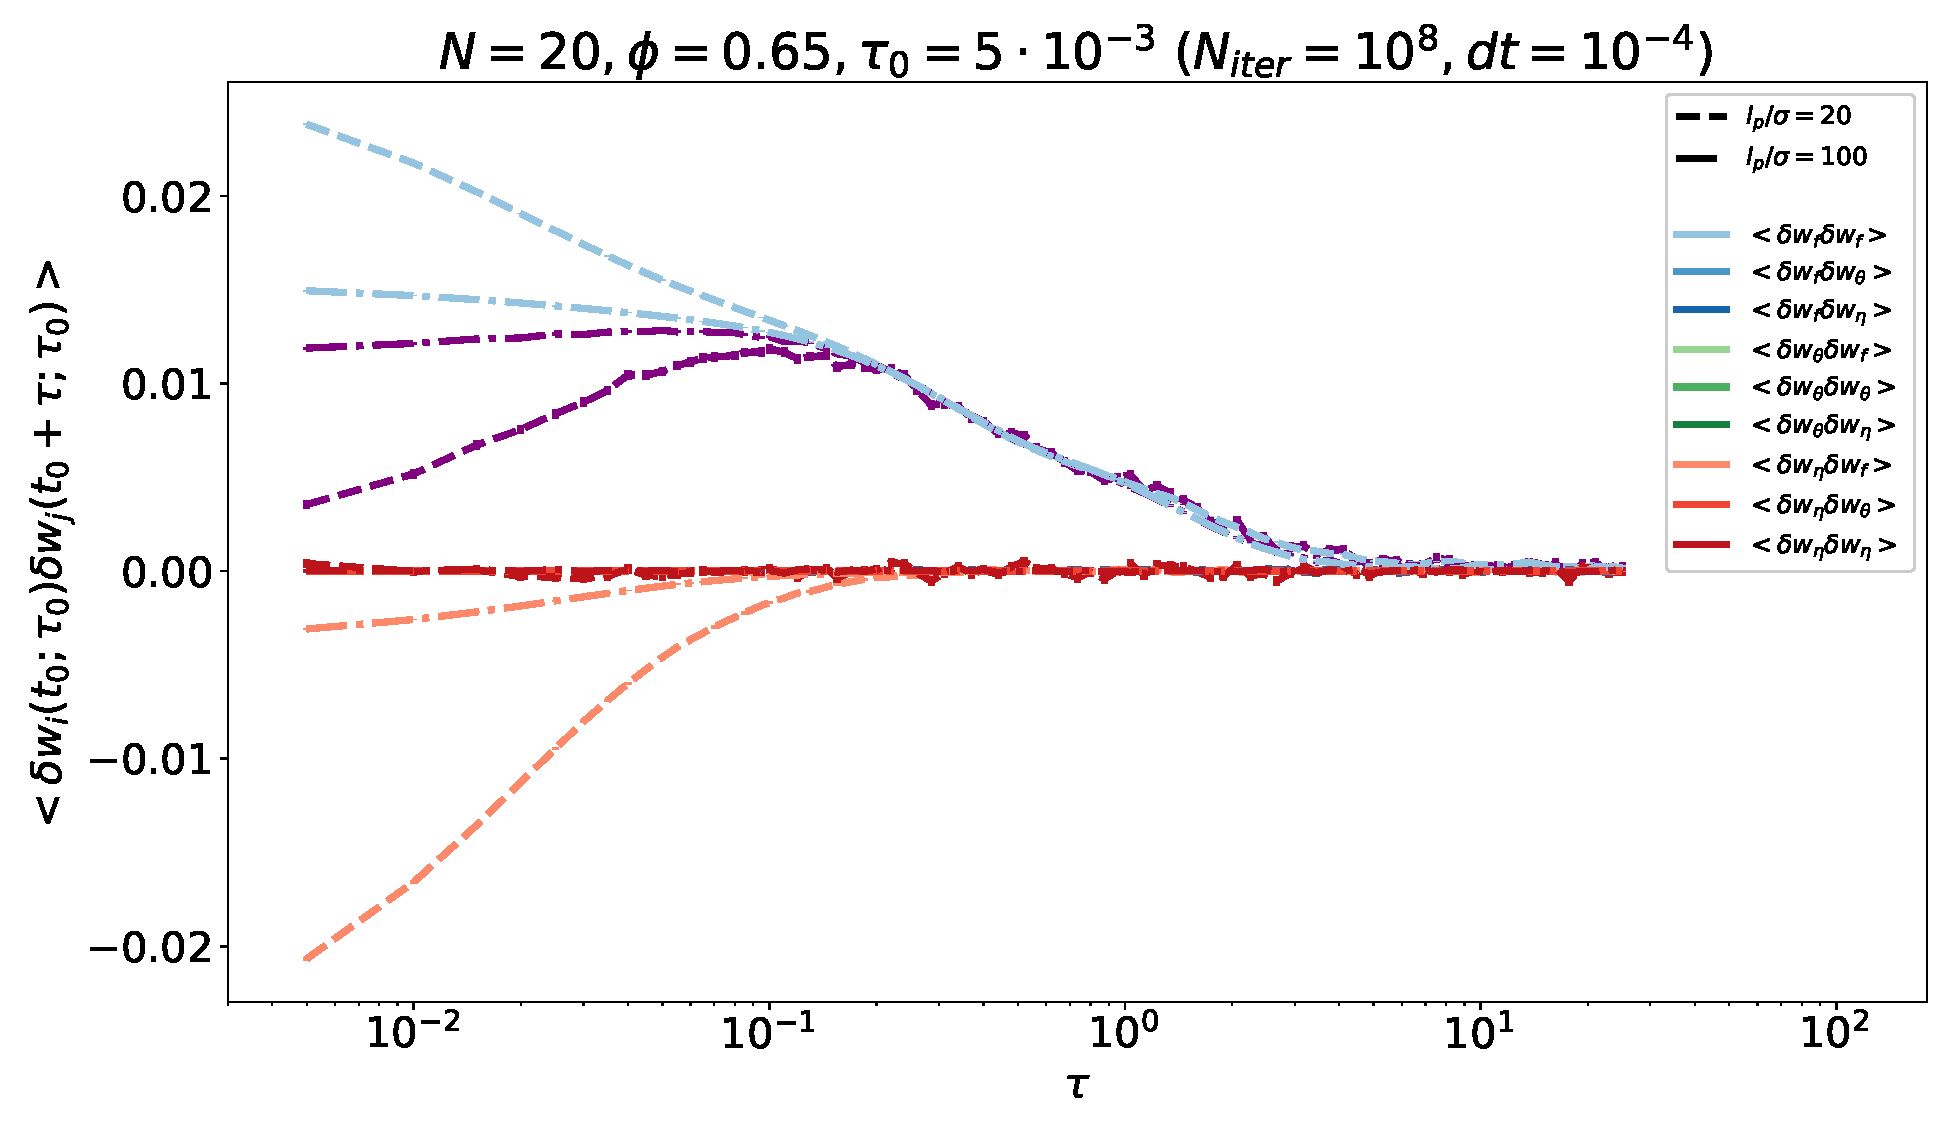
\includegraphics[width=0.7\textwidth]{crossCor_Nm2000_Dk6500_En1000.eps}
\caption{Covariances of active work parts with a delay $\tau$, for $l_p/\sigma = 20$ (dashed lines) and $l_p/\sigma = 100$ (dash-dotted lines). All available intervals but those overlapping with $t_0 \leq 3 l_p/\sigma$ were used to compute the means. These curves are qualitatively independent of the choice of $\tau_0$, this particular choice is a balance between noise reduction and low time resolution. Purple curves correpond to the total active work covariance.}
\label{crossCor}
\end{figure}

We observe that
\begin{itemize}
  \item the covariance of the force part of the active work and itself with a delay $\tau$ is a positive, monotonically decreasing function of $\tau$, with a length scale which increases with persistence length,
  \item the covariance of the noise part of the active work and the force part with a delay $\tau$ is a negative, monotonically increasing function of $\tau$, with a length scale which is qualitatively independent of the persistence length,
  \item the covariance of the active work and itself with a delay $\tau$ is a non-monotonic function of $\tau$, with a peak at $\tau \approx 10^{-1}$.
\end{itemize}

\subsection{Covariance of noise and force part}

\begin{figure}[H]
\centering
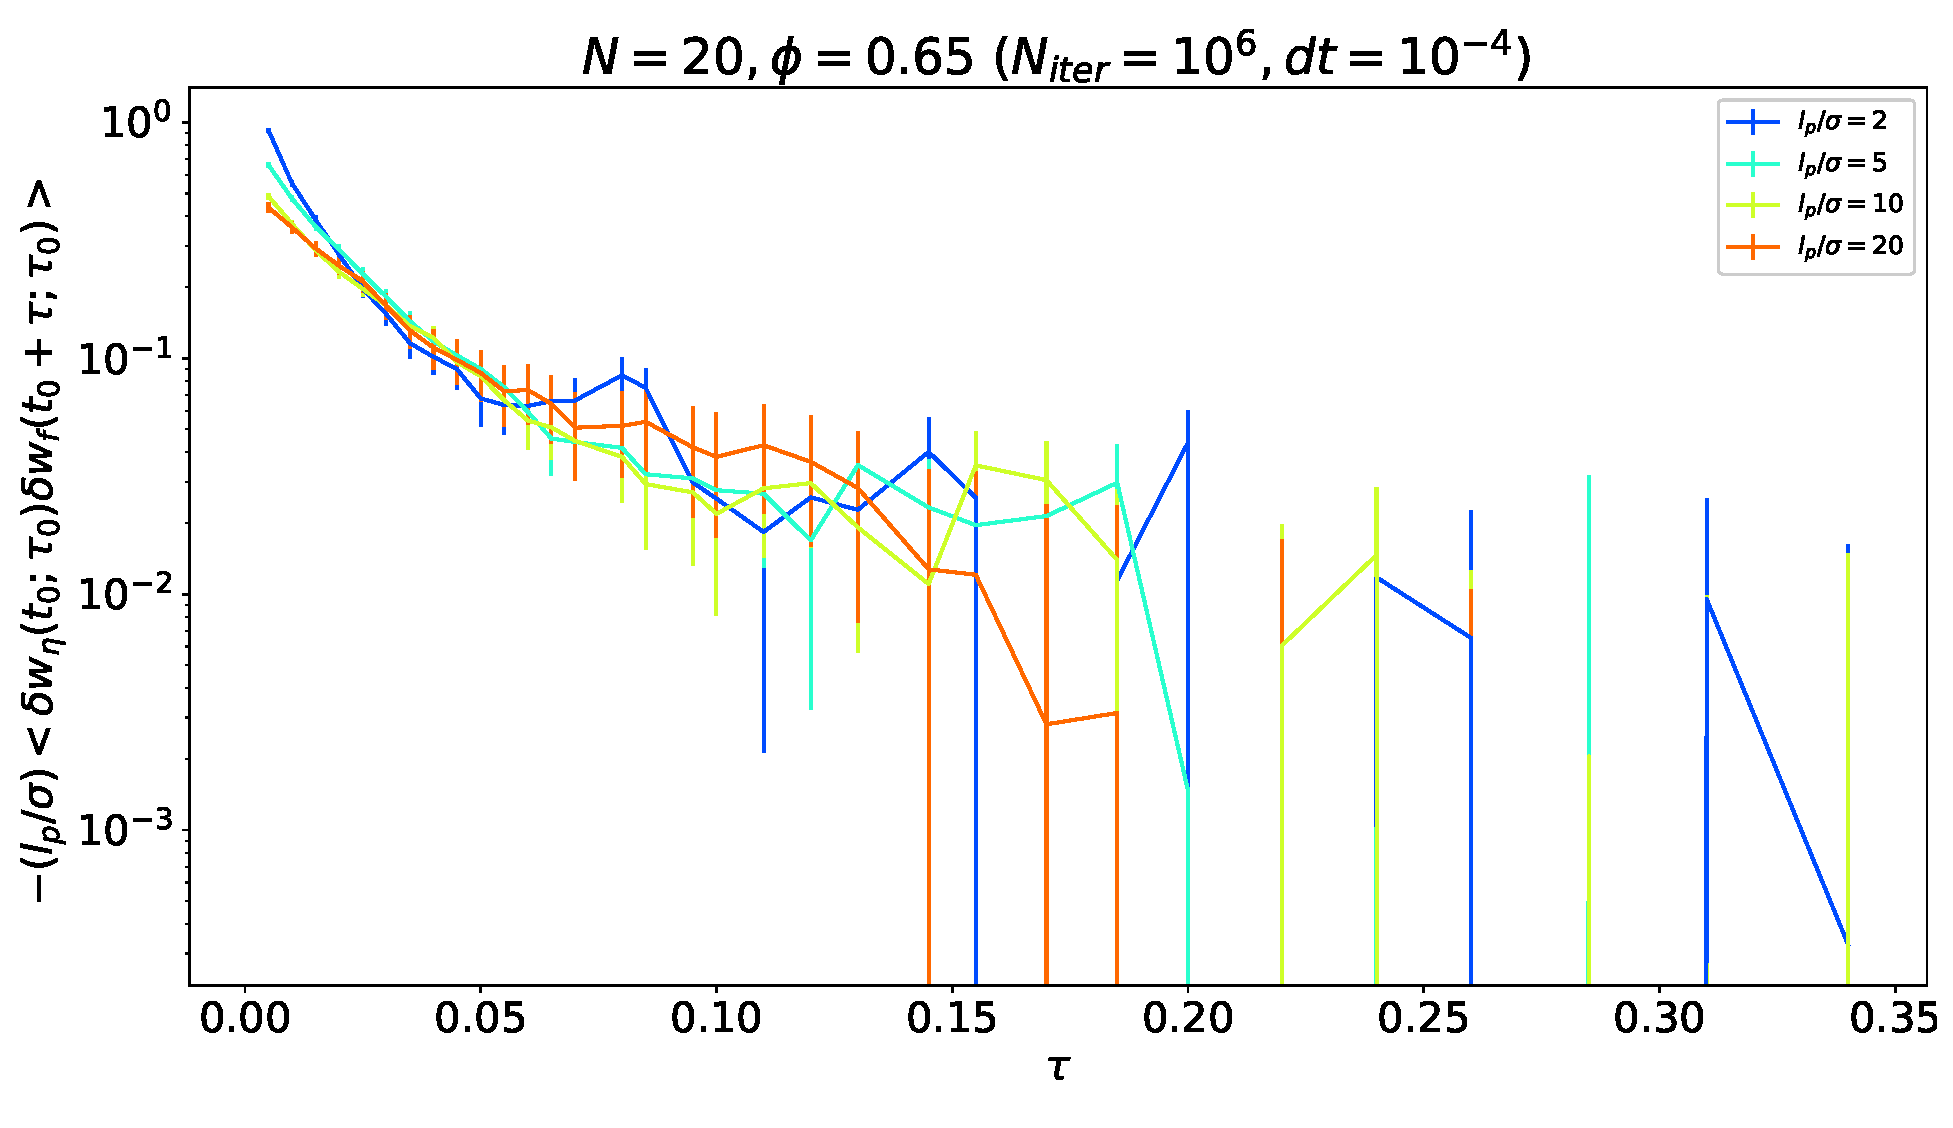
\includegraphics[width=0.7\textwidth]{crossCorNoiseForce_No1000_Dk6500_Em2000.eps}
\caption{Covariance of the noise part of the active workand the force part with a delay $\tau$.}
\label{crossCorNoiseForce}
\end{figure}

We have that for the few values of persistence length tested, $2 \leq l_p/\sigma \leq 20$, the time scale of decrease of the absolute value of $\left<\delta w_{\eta}(t_0; \tau_0) \delta w_f(t_0 + \tau; \tau_0)\right>$ is qualitatively independent of the persistence length (figure \ref{crossCorNoiseForce}).\\

We argue that this time scale is set by the interaction potential. Consider a single particle in a harmonic potential
\begin{align*}
V(\underline{r}(t)) = \frac{1}{2} k \underline{r}(t)^2.
\end{align*}
Motivated by figures \ref{crossCor} and \ref{crossCorNoiseForce}, we assume that $l_p/\sigma \gg \tau_d$, where $\tau_d$ is the relevant time scale of decrease, \ie we can consider that the orientation of the particle is constant. We then have the following equation of motion
\begin{equation}
\dot{\underline{r}}(t) = - \frac{1}{3} \frac{\sigma}{l_p} \nabla V(\underline{r}(t)) + \underline{u}_0 + \sqrt{\frac{2}{3} \frac{\sigma}{l_p}} \underline{\eta}(t).
\end{equation}
We can write
\begin{align*}
\text{d}\left<\left(\underline{\eta}_i(t_0) \cdot \underline{u}_0\right) \, \left(\nabla V(\underline{r}(t_0 + t)) \cdot \underline{u}_0\right)\right> &= \left<\left(\underline{\eta}_i(t_0) \cdot \underline{u}_0\right) \, \left(\underbrace{\nabla^2 V(\underline{r}(t_0 + t))}_{k} \,\text{d}\underline{r}(t_0 + t) \cdot \underline{u}_0\right)\right>\\
&= - k \frac{1}{3} \frac{\sigma}{l_p} \left<\left(\underline{\eta}_i(t_0) \cdot \underline{u}_0\right) \, \left(\nabla V(\underline{r}(t_0 + t)) \cdot \underline{u}_0\right)\right> \, \text{d}t,
\end{align*}
such that
\begin{equation}
\left<\left(\underline{\eta}_i(t_0) \cdot \underline{u}_0\right) \, \left(\nabla V(\underline{r}(t_0 + \tau)) \cdot \underline{u}_0\right)\right> \propto \exp\left(- k \frac{1}{3} \frac{\sigma}{l_p} \tau\right).
\end{equation}

\subsection{Covariance of force part and itself}

According to figure \ref{crossCorForceLP}, we have that $\left<\delta w_f(t_0; \tau_0) \delta w_f(t_0 + \tau; \tau_0)\right>$
\begin{itemize}
  \item decays algebraically at low persistence length $l_p/\sigma = 2$,
  \item decays logarithmically at high persistence length $l_p/\sigma = 20$.
\end{itemize}
We show the buildup of this covariance with increasing persistence length in figure \ref{crossCorForceN}.

\begin{figure}[H]
\centering
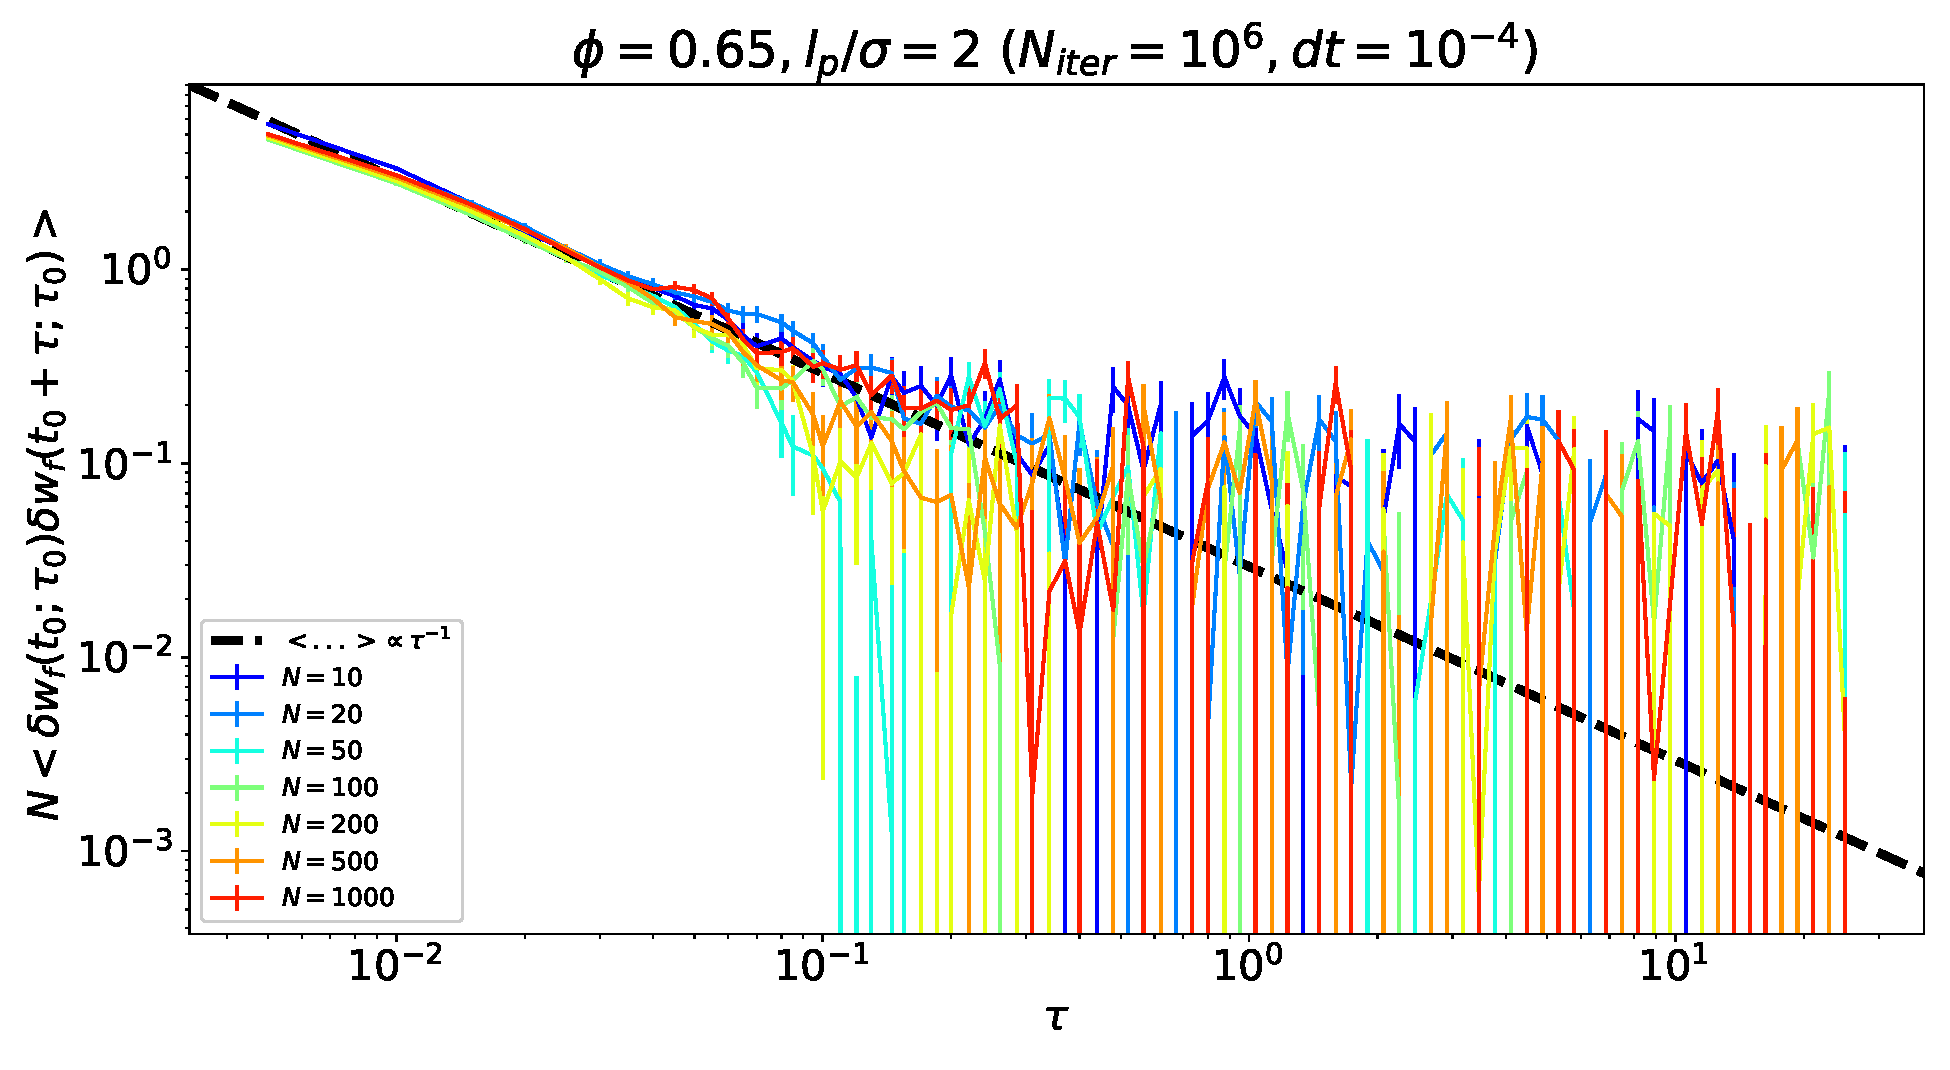
\includegraphics[width=0.49\textwidth]{crossCorForceForce_Dk6500_Ll2000_Em2000.eps}
\hfill
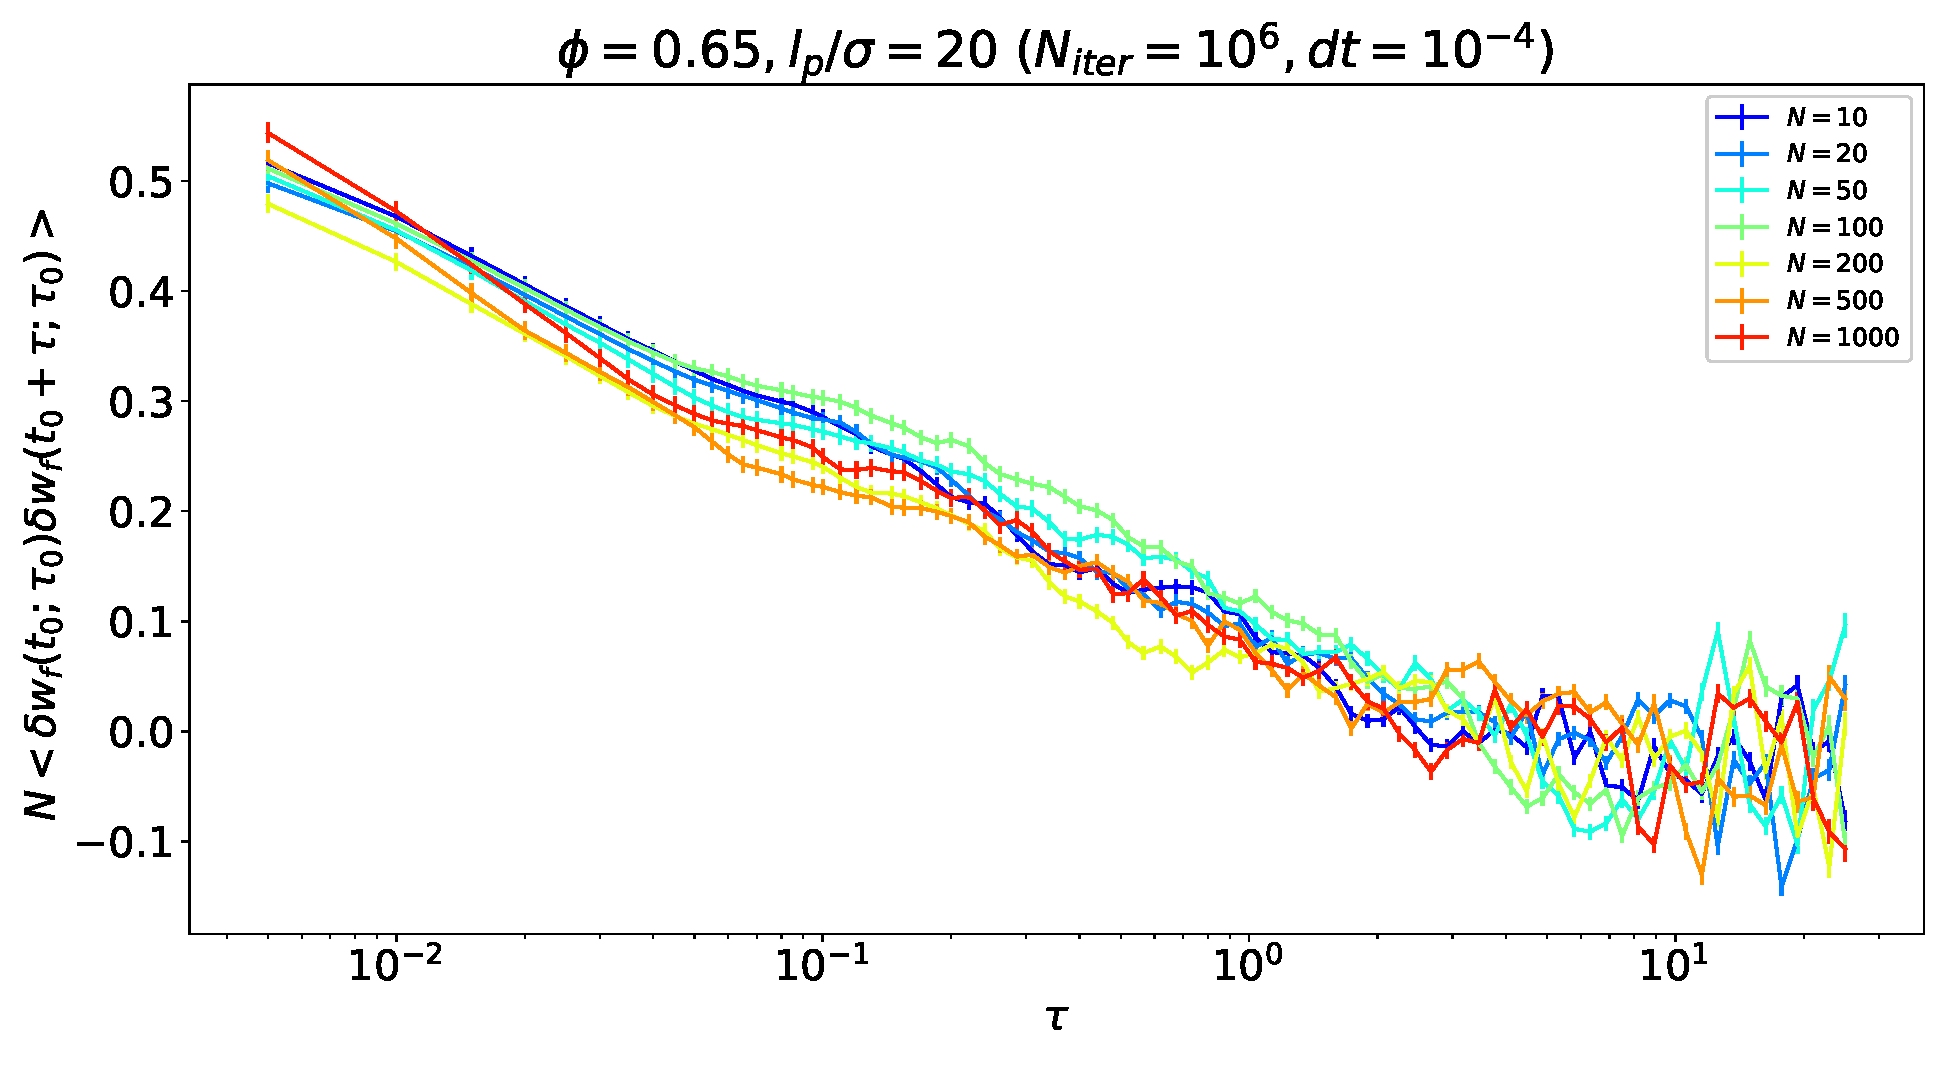
\includegraphics[width=0.49\textwidth]{crossCorForceForce_Dk6500_Lm2000_Em2000.eps}
\caption{Covariance of the force part of the active work and itself with a delay $\tau$ for $l_p/\sigma = 2$ (left) and $l_p/\sigma = 20$ (right).}
\label{crossCorForceLP}
\end{figure}

\begin{figure}[H]
\centering
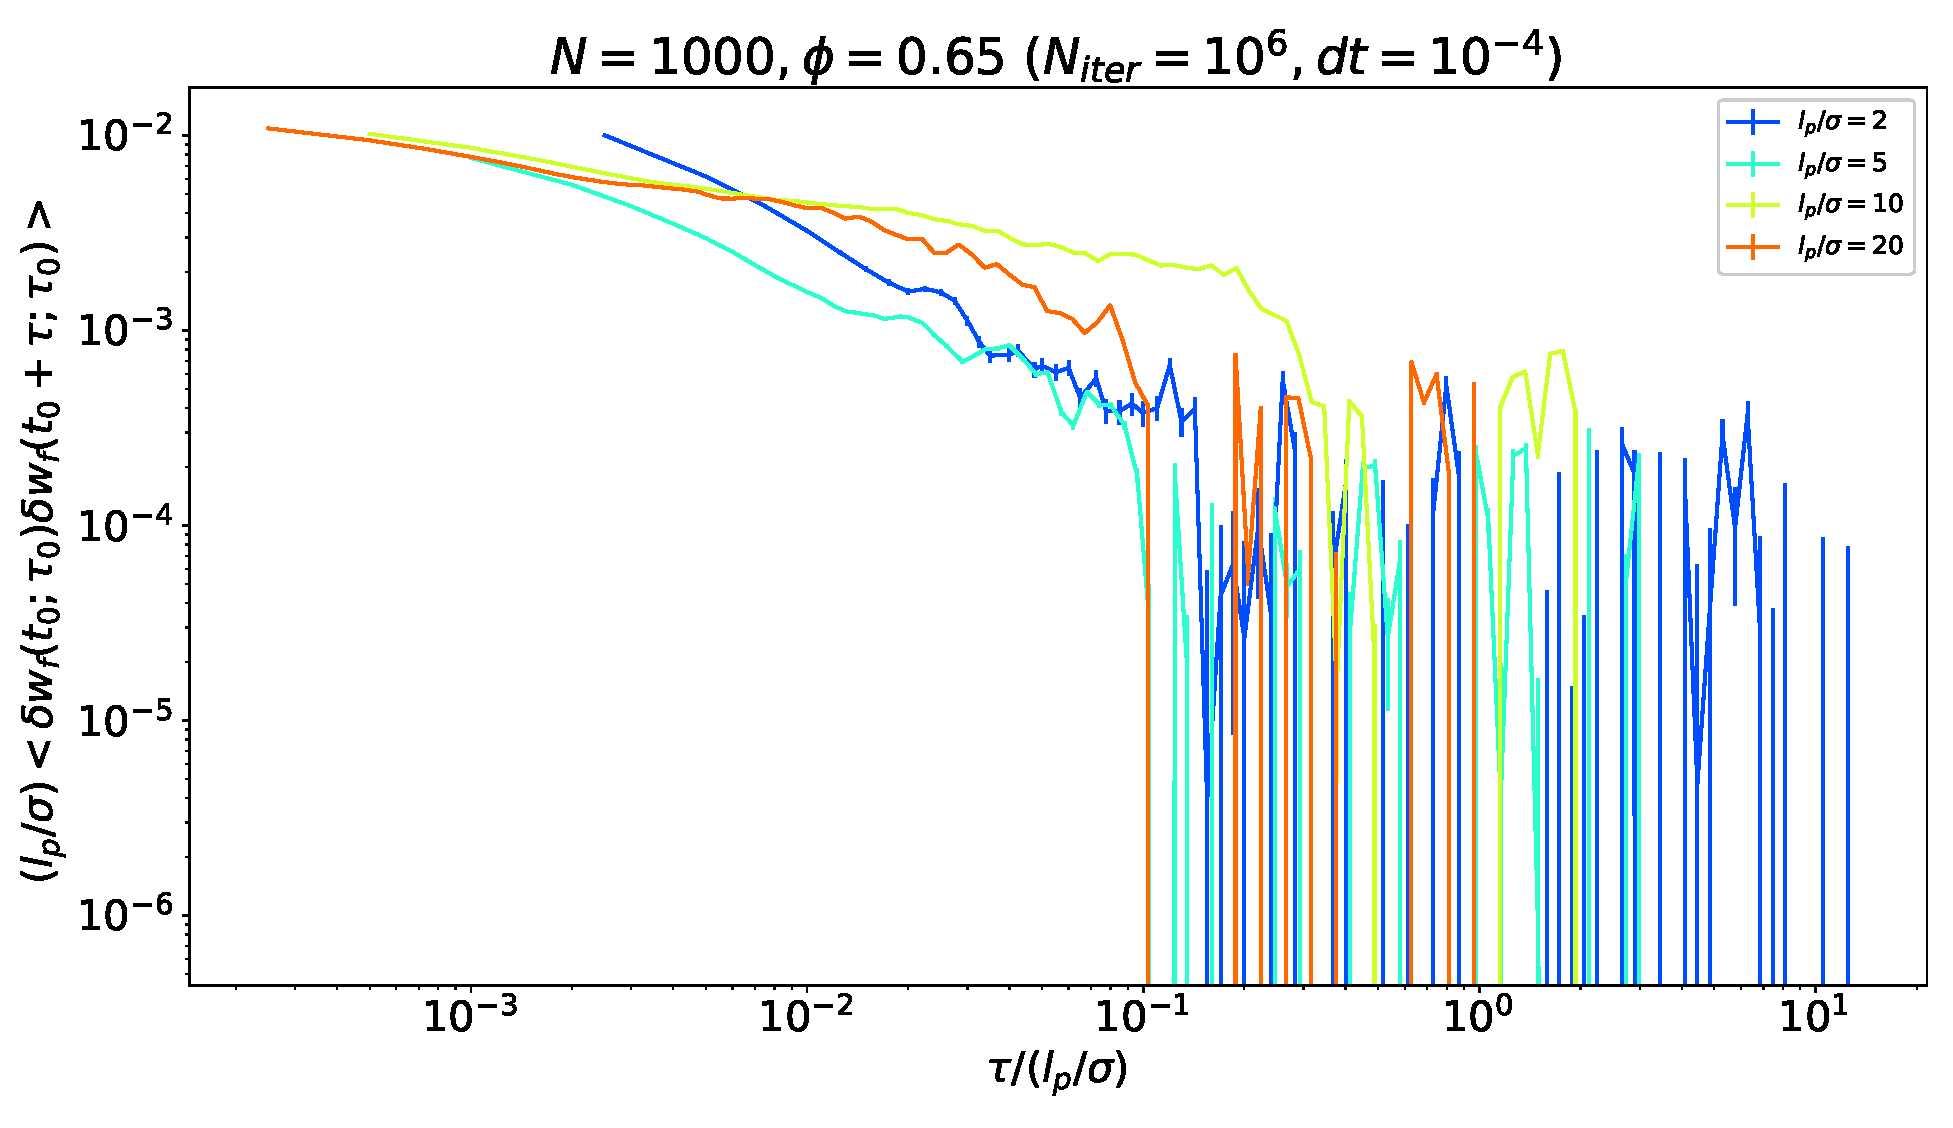
\includegraphics[width=0.7\textwidth]{crossCorForceForce_No1000_Dk6500_Em2000.eps}
\caption{Covariance of the force part of the active work and itself with a delay $\tau$ for $2 \leq l_p/\sigma \leq 20$ at $N=10^3$ particles.}
\label{crossCorForceN}
\end{figure}

According to \cite{tociu_how_2018}, the mean force part of the normalised rate of active work in steady state is linked to the structure of the liquid,
\begin{equation}
\left<w_f\right> = \phi \int g(\underline{r}) \left\{[\nabla V(\underline{r})]^2 - \frac{2}{3}\frac{\sigma}{l_p} \nabla^2 V(\underline{r})\right\} \, \text{d}\underline{r} + \phi^2 \iint g_3(\underline{r}, \underline{r}^{\prime}) \nabla V(\underline{r}) \cdot \nabla V(\underline{r}^{\prime}) \, \text{d}\underline{r} \, \text{d}\underline{r}^{\prime},
\end{equation}
where $g$ and $g_3$ are the two- and three-body density correlations among particles.\\

Maybe then is the decay of $\left<\delta w_f(t_0; \tau_0) \delta w_f(t_0 + \tau; \tau_0)\right>$ linked to the relaxation of the structure. We have that at $l_p/\sigma = 2$ the system resembles an homogeneous liquid, while at $l_p/\sigma = 20$ denser regions -- clusters -- appear (figure \ref{screenshots}). Moreover, clusters are expected to get denser as the persistence length increases, and particles move more slowly in denser regions \cite{cates_motility-induced_2015}. We can thus imagine that the buildup of the covariance of the force part of the active work and itself with a delay $\tau$ is directly linked to this changing dynamical picture with increasing persistence length. Such a link remains to be demonstrated.

\begin{figure}[H]
\centering
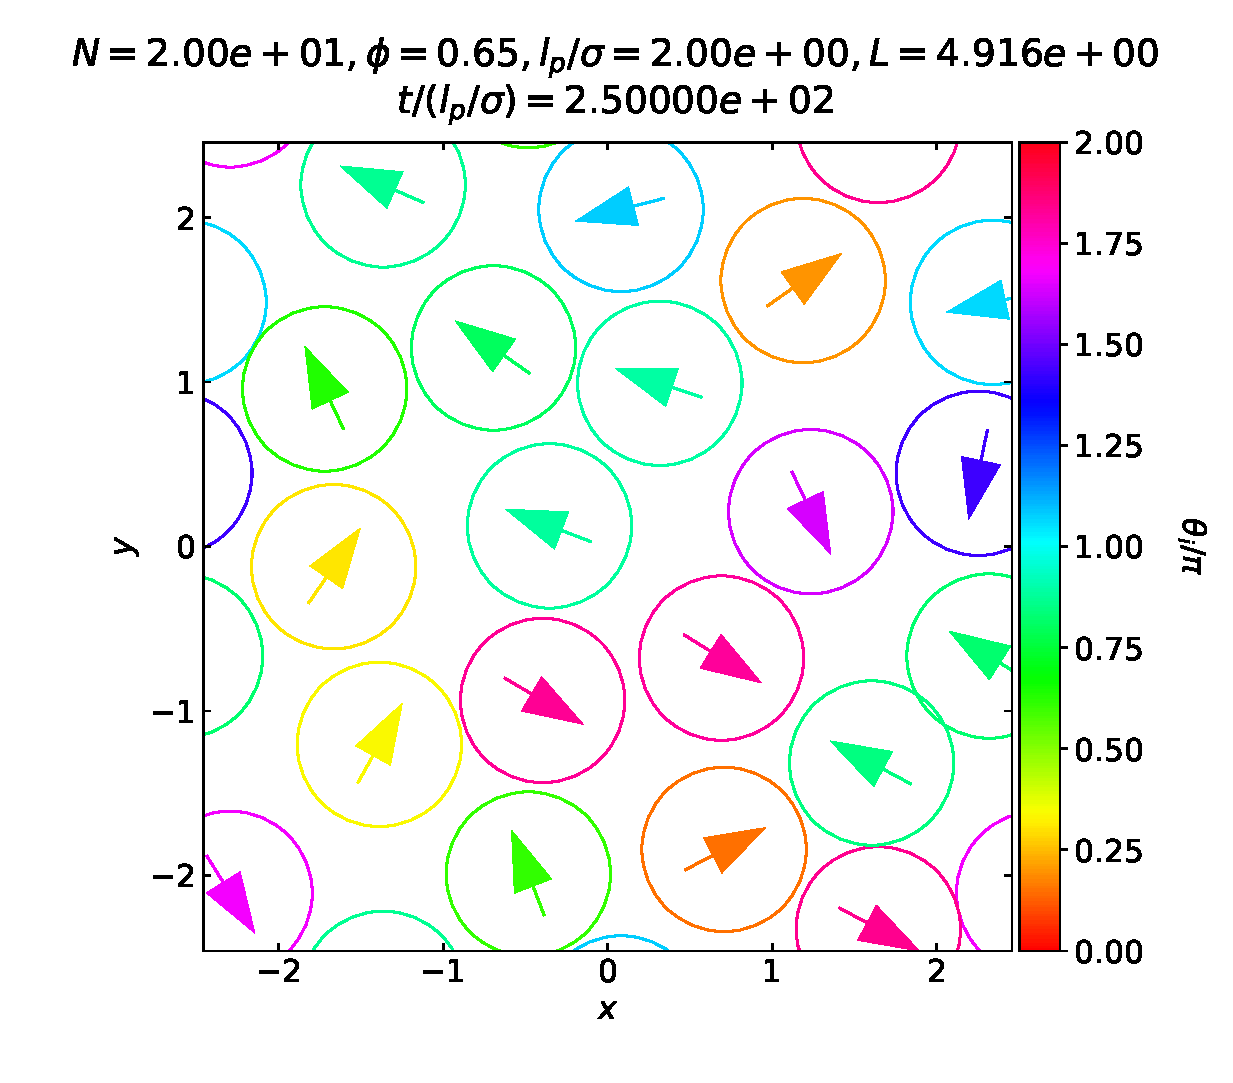
\includegraphics[width=0.49\textwidth]{o_Nm2000_Dk6500_Ll2000.eps}
\hfill
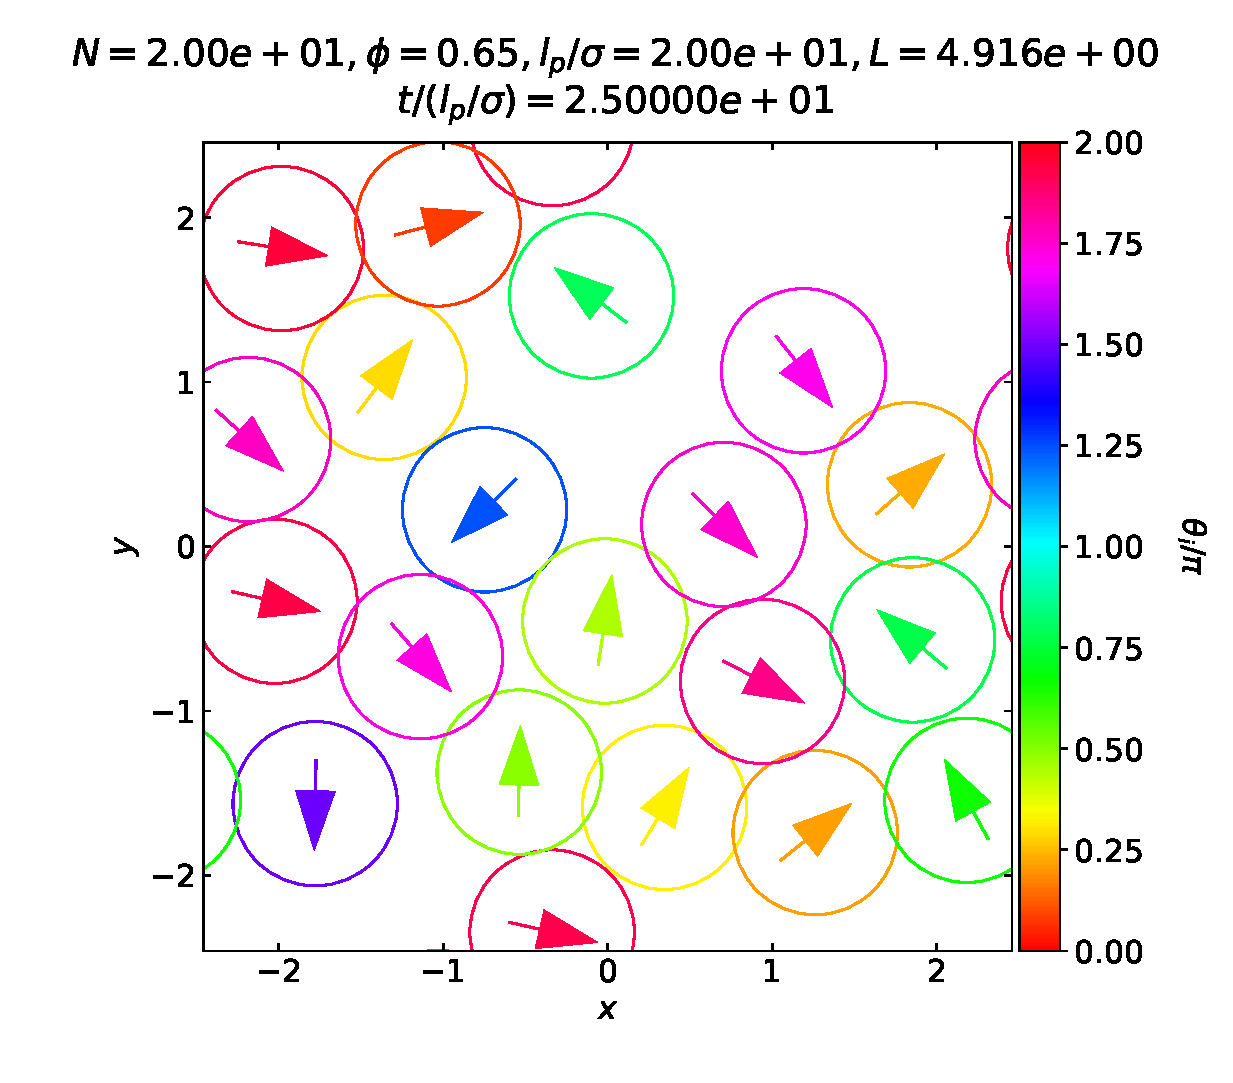
\includegraphics[width=0.49\textwidth]{o_Nm2000_Dk6500_Lm2000.eps}
\caption{Screenshots of the system for $l_p/\sigma = 2$ (left) and $l_p/\sigma = 20$ (right). Colors refer to the orientation of the particles.}
\label{screenshots}
\end{figure}

\section{Order and active work}

We compute the correlation function between the flucutations of the order parameter norm at time $t_0$ and the flucutations of the normalised rate of active work on the interval $[t_0; t_0 + \tau]$ (figure \ref{Cawo}),
\begin{equation}
C^{(a)}_{wo}(\tau) = \frac{\left<\delta w(t_0; \tau) \, \delta |\underline{\nu}(t_0)|\right>}{\sqrt{\left<\delta w(t_0; \tau)^2\right> \, \left<\delta |\underline{\nu}(t_0)|^2\right>}}.
\label{eqCawo}
\end{equation}

\begin{figure}[H]
\centering
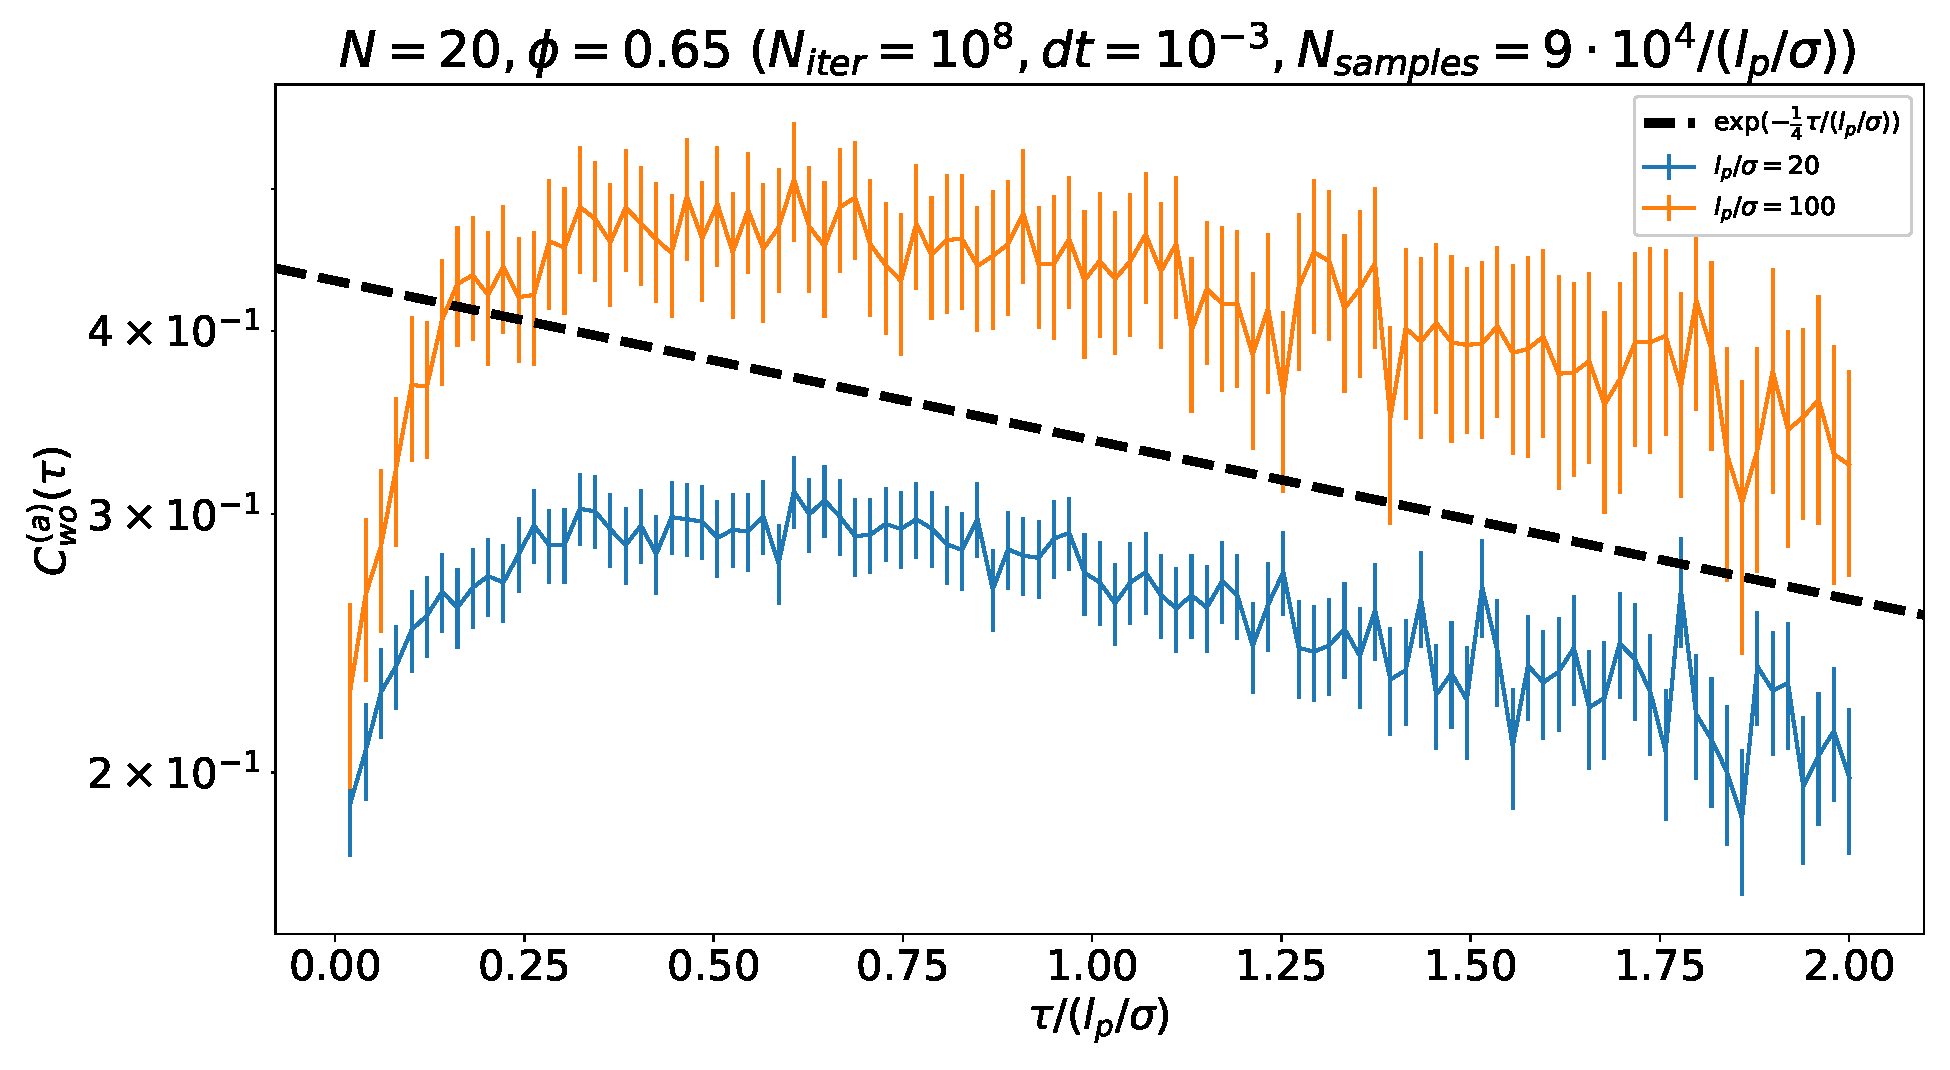
\includegraphics[width=0.7\textwidth]{corWorkOrderAve_Nm2000_Dk6500_Em1000.eps}
\caption{Correlation function between the flucutations of the order parameter norm at time $t_0$ and the flucutations of the normalised rate of active work on the interval $[t_0; t_0 + \tau]$.}
\label{Cawo}
\end{figure}

First of all, we note that this correlation function is non-monontic. This can rationalised by the fact that the variance of the active work,
\begin{align*}
\tau \mapsto \left<\delta w(t_0; \tau)^2\right>,
\end{align*}
is a monotonically decreasing function of $\tau$.\\

We have that the fluctuations of the normalised rate of active work $w$ over an interval $[t_0; t_0 + \tau]$ are positively correlated with fluctuations of the order parameter $|\underline{\nu}|$ at the beginning of this interval. This may indicate that positive fluctuations of the order parameter norm at a given time leads to an increased active work at following times. This can be explained by the fact that nematically ordered particles -- \ie high $|\underline{\nu}|$ -- have fewer collisions, so that active forces translates more efficiently into particle motion \cite{nemoto_optimizing_2019}.\\

We also note that these correlations decay on a length scale larger than the rotational diffusion time -- the dashed black line is here for illustration purposes and does not reflect any theoretical predicition. Furthermore, we have that the correlations between the averaged active work and the order parameter norm are higher for $l_p/\sigma=100$ than for $l_p/\sigma = 20$ -- this may however be due, in part or completely, to the fact that the variance of the active work is higher in the latter.\\

We also compute the covariance of the order parameter norm and the normalised rate of active work with a delay $\tau$ (figure \ref{covWorkOrder}),
\begin{equation}
\tau \mapsto \left<\delta |\underline{\nu}(t_0)| \delta w(t_0 + \tau; \tau_0)\right>,
\end{equation}
which is linked to the numerator in equation \ref{eqCawo} by summation over the interval $[t_0; t_0 + \tau]$.

\begin{figure}[H]
\centering
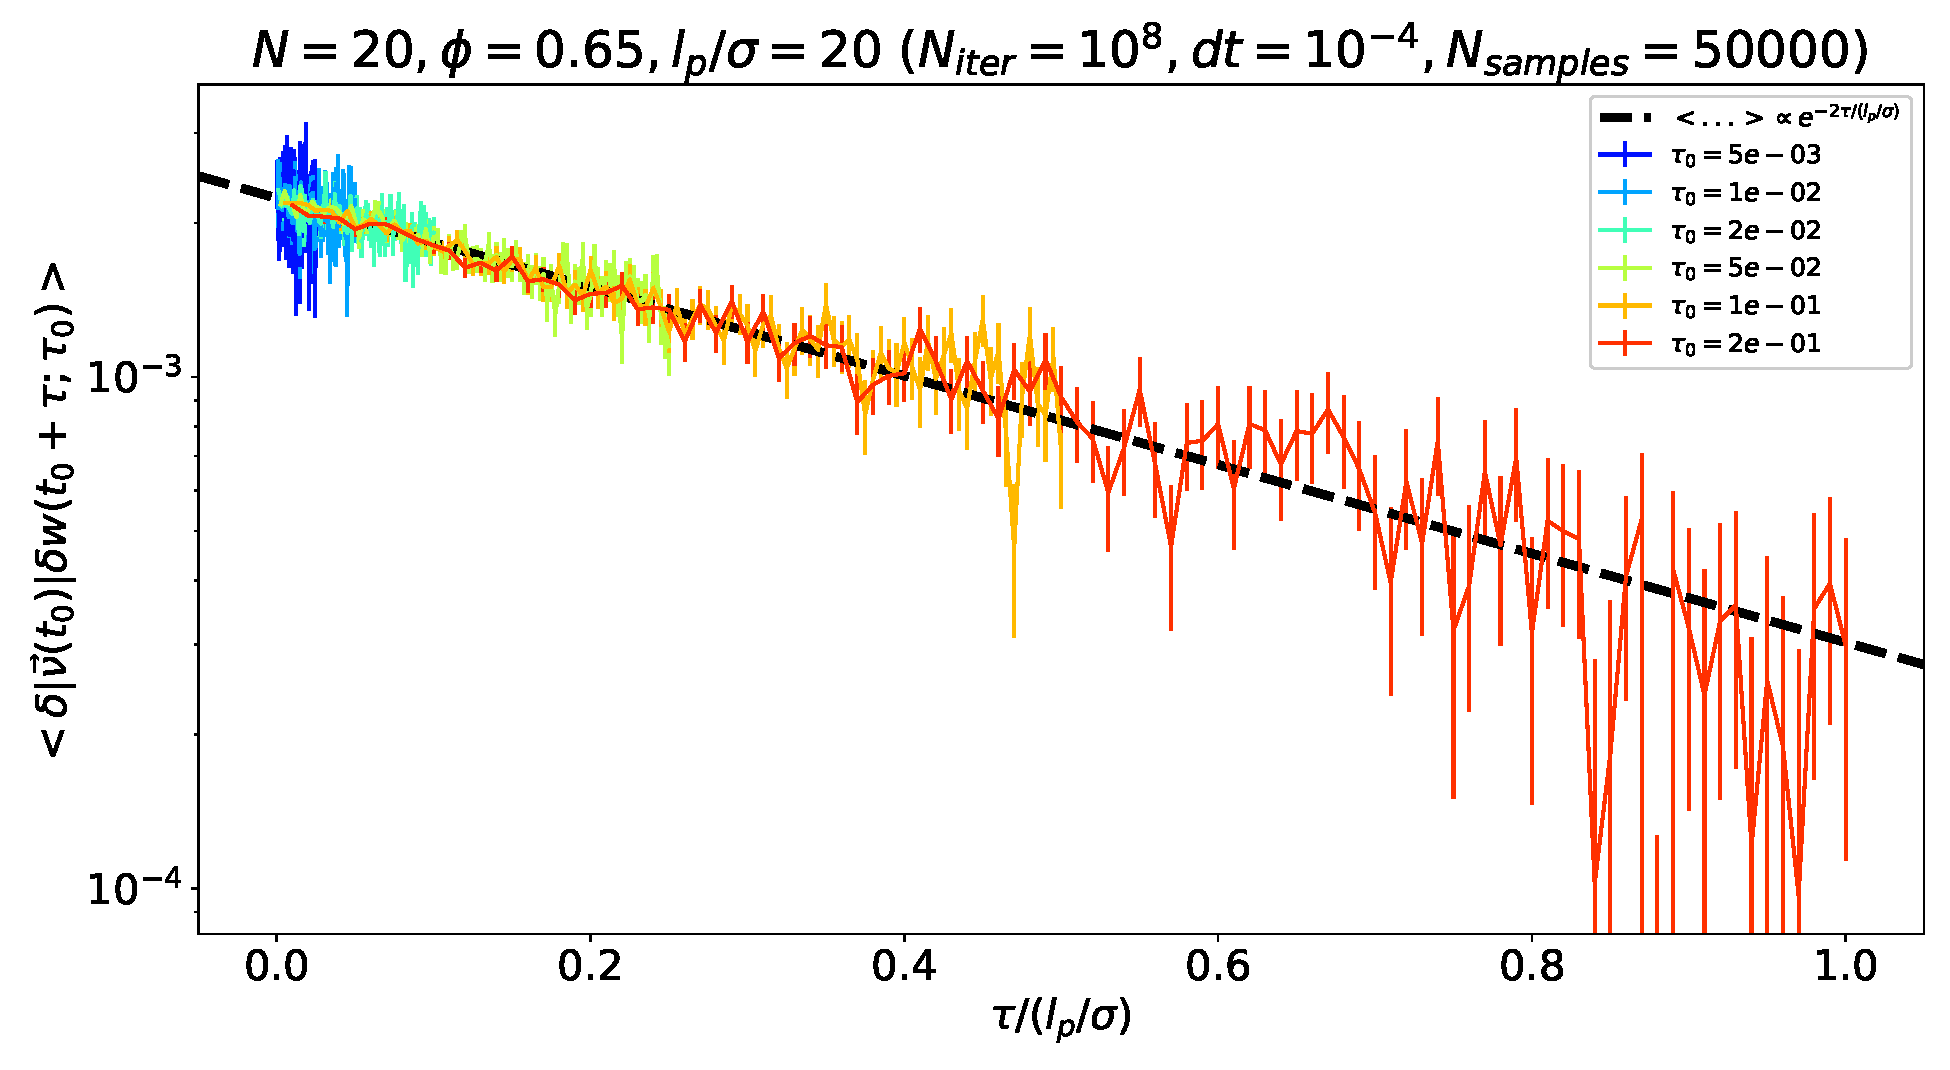
\includegraphics[width=0.49\textwidth]{corWorkOrderIns_Nm2000_Dk6500_Lm2000_Em1000_Ip5000.eps}
\hfill
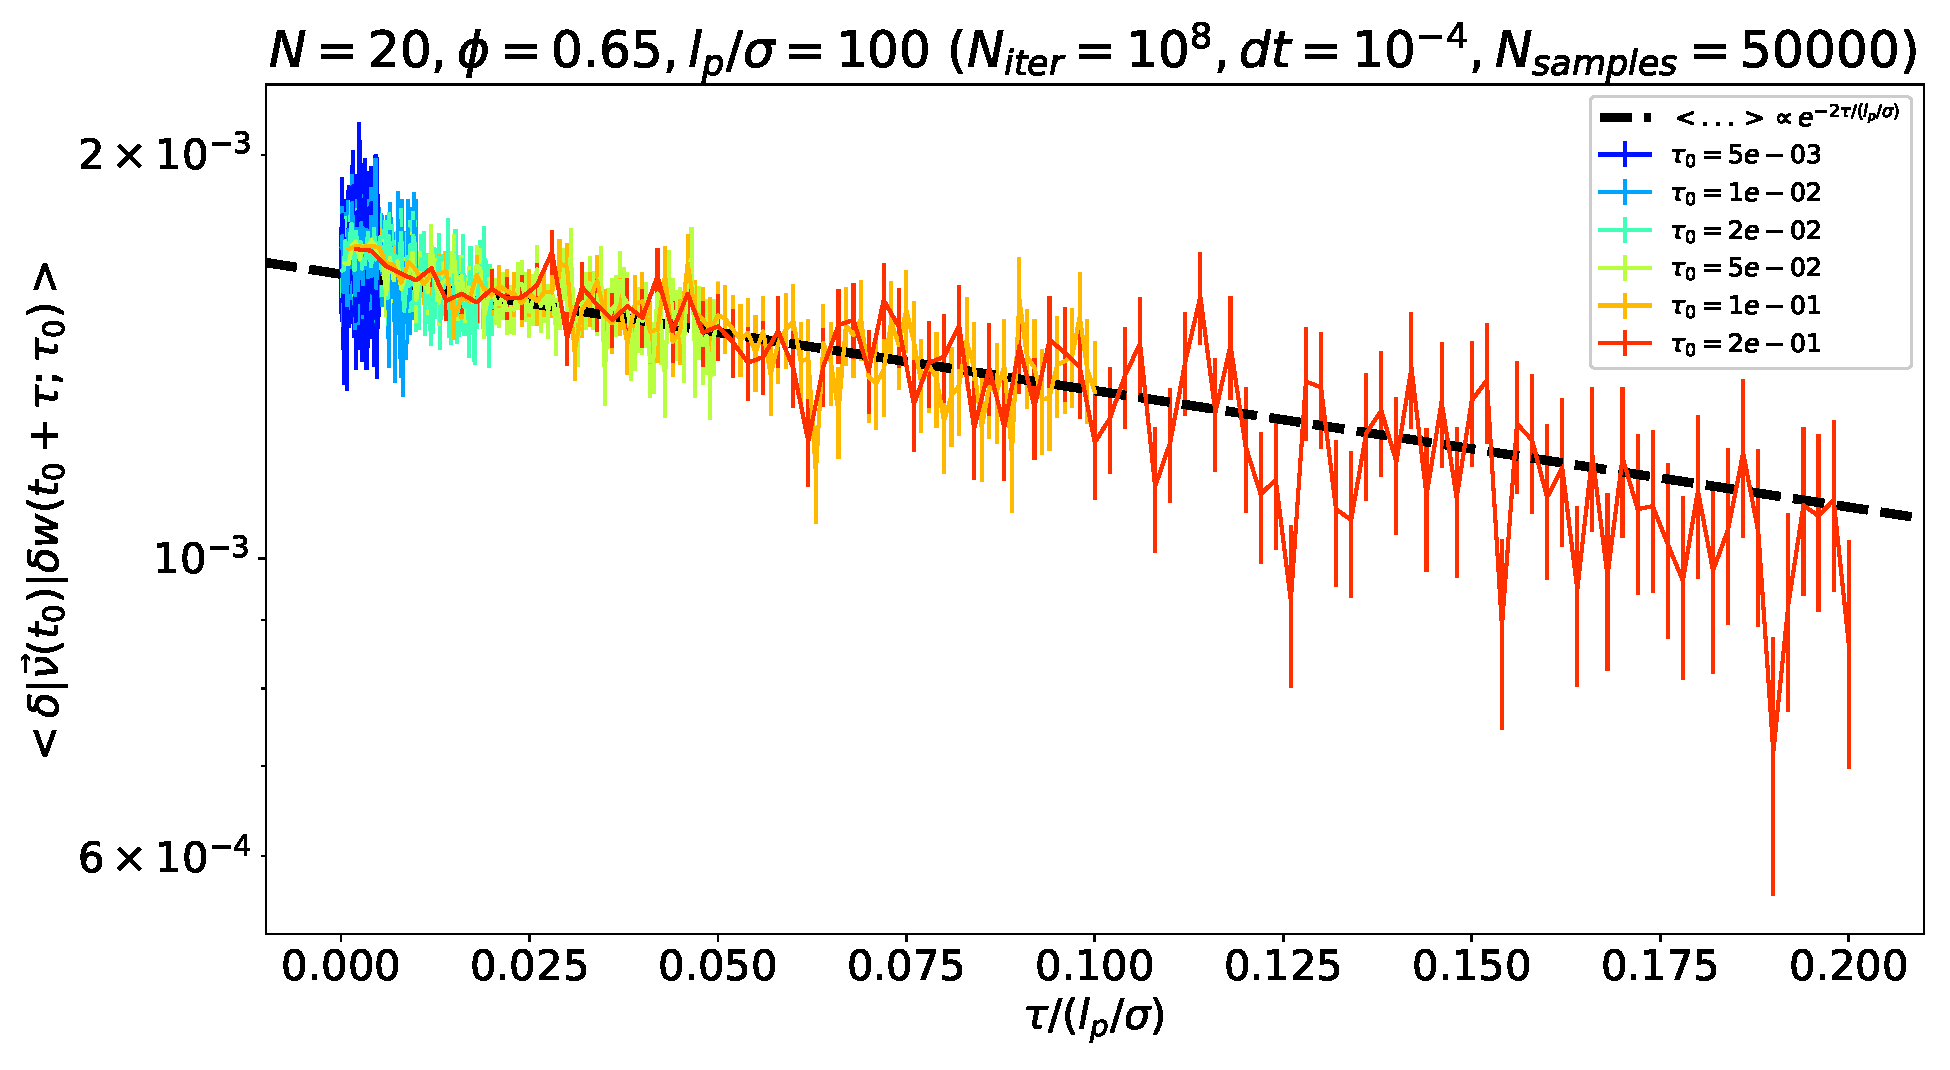
\includegraphics[width=0.49\textwidth]{corWorkOrderIns_Nm2000_Dk6500_Ln1000_Em1000_Ip5000.eps}
\caption{Covariance of the order parameter norm and the normalised rate of active work with a delay $\tau$ for $l_p/\sigma = 20$ (left) and $l_p/\sigma = 100$ (right).}
\label{covWorkOrder}
\end{figure}

We have a monotonic decrease of this covariance with a length scale $\sim \frac{1}{2} \frac{l_p}{\sigma}$ for both tested values of the persistence length.

%%%%%%%%%%%%%%
% REFERENCES %
%%%%%%%%%%%%%%

\bibliographystyle{unsrtnat}
{\renewcommand{\bibname}{References}\bibliography{ref}}

\end{document}
